\subsection{Mercatorprojektion}
\label{sec:mercator} 
Die Mercatorprojektion ist eine winkeltreue Zylinderprojektion. Sie erreicht dabei nie Pole.
Die Längengrade verlaufen in dieser Projektion parallel und haben den gleichen Abstand zueinander.
Die Breitengrade sind ebenfalls parallel zueinander haben aber unterschiedliche Abstände.
Die Verzerrung nimmt mit Polnähe zu, das heißt, dass die Karte zu den Polen hin gestreckt wird.\\

\begin{figure}[hbtp]
\centering
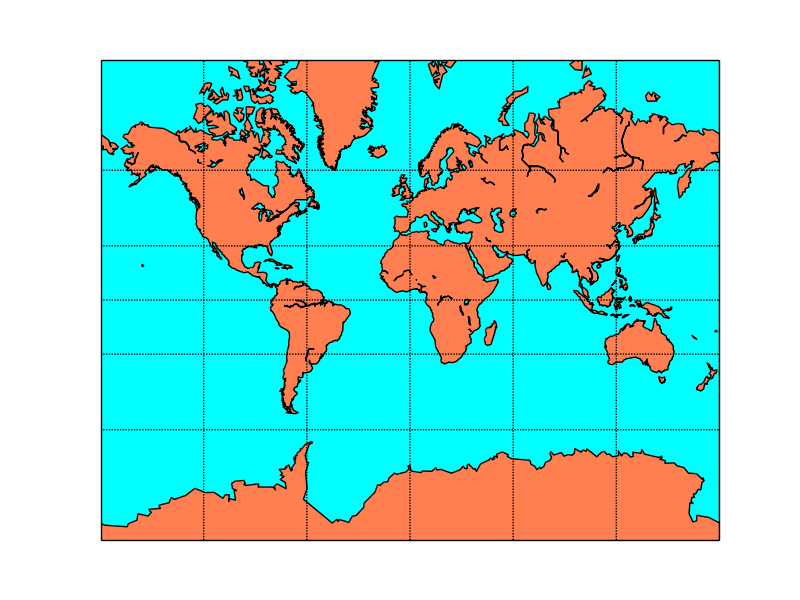
\includegraphics[scale=0.5,origin=c]{/Users/student/seminar/Kartendarstellungen/seminar/merc} \caption{Mercatorprojektion}
\end{figure}
\newpage 